
\section{Evaluation}
\begin{frame}
	
	\frametitle{ Evaluation of Proposed Approach }
	\framesubtitle{Performance Measures}

		\begin{itemize}
			\item<1->  $\mathit{Precision} =$ $ \mathit{\frac{\#\ of\ correct\ predictions}{\#\ of\ total\ predictions}}$ is the fraction of the produced predictions that are correct (i.e., a full match occurred within the prediction interval).   
			
			\item<2-> $\mathit{Spread} =end(I) -start(I)$ is the width of the prediction interval $I$.  
			
				\item<3->  $\mathit{Cumulative\ communication}$:
		   number of messages, which are required to perform the distributed online learning modes to synchronize the prediction models.
		\end{itemize}

\end{frame}



%\begin{frame}
%	
%	\frametitle{Initial Experimental Results }
%	\framesubtitle{Setup}
%1	analytical \& theoretical analysis 
% 2 evaluation with synthetic datastest \& 3 real datasets and grouping thing  
% then initial results 
%	
%\end{frame}


\begin{frame}
	
	\frametitle{Empirical evaluation }
	\framesubtitle{Experimental Setup}
\begin{itemize}
	\item<1-> Synopses over raw AIS messages in Brest, France: 1 October 2015 to 31 March 2016 (ais\_brest\_synopses.json). 
	
	\item<1->$ 4,684,444$ derived critical points.
	
	\item<1->  $\approx5000$ vessels.
	\item<2> Used patterns are:
	$\mathcal{P}_1=Sailing$  \& \newline
	$\mathcal{P}_2=$\textit{changeInHeading; gapStart; gapEnd; changeInHeading}.
\end{itemize}
	
\end{frame}


\begin{frame}
	
	\frametitle{Empirical evaluation }
	\framesubtitle{Precision scores with respect to the number of input events over time for $\mathcal{P}_1$}
	
	\begin{center}
		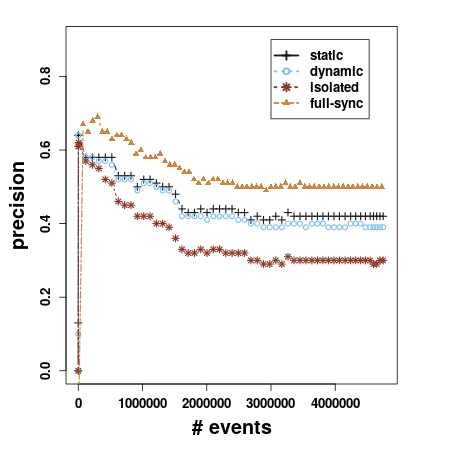
\includegraphics[width=.8\textwidth,height=.7\linewidth]{figures/precision_p1.png}
		.
	\end{center}
	
\end{frame}

\begin{frame}
	
	\frametitle{Empirical evaluation }
	\framesubtitle{Precision scores with respect to the number of input events over time for $\mathcal{P}_1$}
	
	\begin{itemize}
		\item<1-> All methods of distributed learning outperform the isolated prediction model
		
		\item<1->  The hypothetical method of full continuous synchronization has the highest precision rates.
		\item<1-> The static and dynamic synchronization schemes have close precision scores
		
	\end{itemize}
	
\end{frame}




\begin{frame}
	
	\frametitle{Empirical evaluation }
	\framesubtitle{Average spread value for $\mathcal{P}_1$}
	
	\begin{center}
		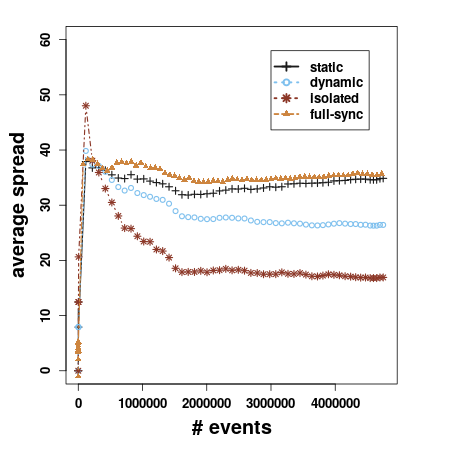
\includegraphics[width=.8\textwidth,height=.7\linewidth]{figures/spread_p1.png}
		.
	\end{center}
	
\end{frame}

\begin{frame}
	
	\frametitle{Empirical evaluation }
	\framesubtitle{Average spread value for $\mathcal{P}_1$}
	
\begin{itemize}
	\item<1-> The spread is higher for the distributed learning based methods comparing to the isolated approach
	
	\item<1-> The average spread is decreasing over time until convergence,which may explains the drop in the precision scores from the beginning until reaching the convergence.
	
\end{itemize}
	
\end{frame}




\begin{frame}
	
	\frametitle{Empirical evaluation }
	\framesubtitle{Commutative communication with respect to the number of input events over time for $\mathcal{P}_1$}
	
	\begin{center}
		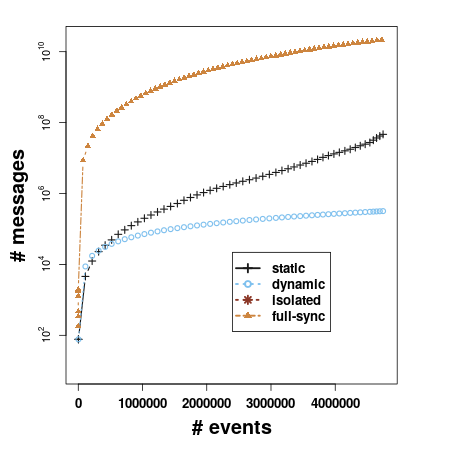
\includegraphics[width=.8\textwidth,height=.7\linewidth]{figures/messages_p1.png}
		.
	\end{center}
	
\end{frame}

\begin{frame}
	
	\frametitle{Empirical evaluation }
	\framesubtitle{Commutative communication with respect to the number of input events over time for $\mathcal{P}_1$}
	
	\begin{itemize}
		\item<1-> A larger amount of communication is required for the continuous synchronization comparing to the static and dynamic approaches
		
		\item<1-> We can reduce the communication overhead by applying the dynamic synchronization protocol (a reduction by a factor of 100) comparing to the static synchronization scheme
	
\end{itemize}
\end{frame}



\begin{frame}
	
	\frametitle{Empirical evaluation }
	\framesubtitle{Precision scores of $\mathcal{P}_2$  for \textit{PLEASURE CRAFT} vessels}
	
	\begin{center}
		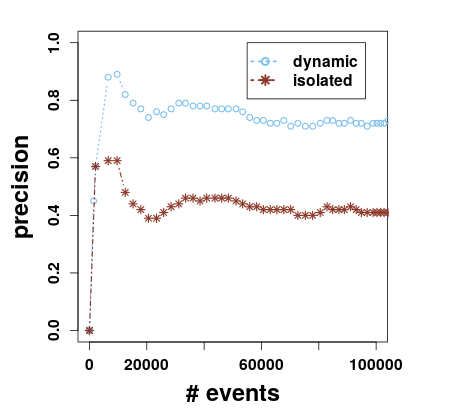
\includegraphics[width=.8\textwidth,height=.7\linewidth]{figures/precision_p2.png}
		.
	\end{center}
	
\end{frame}

\begin{frame}
	
	\frametitle{Empirical evaluation }
	\framesubtitle{Precision scores of $\mathcal{P}_2$  for \textit{PLEASURE CRAFT} vessels}
	
	\begin{itemize}
	\item<1-> For the second, more complex pattern ($\mathcal{P}_2$), we have found that the precision was worse for a distributed model generated over all vessels than in the model created for each vessel in isolation
	
\item<1-> 	So we only enabled the synchronization of the prediction models associated with vessels that belong to the same vessel class e.g., \textit{PLEASURE CRAFT}
	
\end{itemize}
	
\end{frame}

\begin{frame}
	
	\frametitle{ Next steps }
	
	
	\begin{itemize}
		\item<1->  Interface definition with Elias for independent updates 
		
		\item<1-> Evaluation on synthetic data 
		
		\item<1->  Analysis of distributed learning  effects
		\item<1-> Performance measurements on datAcron cluster 
	    \item<1-> Prediction intervals with time information
	
	\end{itemize}
	
\end{frame}
